\section{Función generadora de momentos}
\label{sec:mgf}\label{sec:3.4}

La función generadora de momentos (FGM) es una herramienta que codifica toda la
información de una distribución de probabilidad en una única función.

\begin{definicion}[Función generadora de momentos]
Sea $X$ una variable aleatoria. Su \emph{función generadora de momentos} (FGM) es
\begin{align}
 \label{eq:2.8.11}
 M_X(t) = E\!\left[e^{tX}\right].
\end{align}
Si $X$ es discreta con función de probabilidad $f$,
\begin{align}
 M_X(t) = \sum_x e^{tx} f(x).
\end{align}
Si $X$ es continua con función de densidad $f$,
\begin{align}
 M_X(t) = \int_{-\infty}^{\infty} e^{tx} f(x)\,dx.
\end{align}
\end{definicion}

La FGM existe si la integral o suma converge en un entorno abierto de $t=0$.

\subsection{Momentos a partir de la FGM}

\begin{teorema}[Derivadas y momentos]
Si $M_X(t)$ es la FGM de $X$, entonces para todo $n \in \mathbb{N}$,
\begin{align}
 \label{eq:2.8.12}
 E\!\left[X^n\right] = M_X^{(n)}(0) = \left.\frac{d^n M_X(t)}{dt^n}\right|_{t=0}.
\end{align}
\end{teorema}

\begin{proof}
Intercambiando derivada y esperanza (bajo condiciones de regularidad):
\begin{align}
 M_X^{(n)}(t) = \frac{d^n}{dt^n}E[e^{tX}] = E\!\left[\frac{d^n}{dt^n}e^{tX}\right]
 = E\!\left[X^n e^{tX}\right].
\end{align}
Evaluando en $t=0$ obtenemos $M_X^{(n)}(0) = E[X^n]$.
\end{proof}

\subsection{Unicidad y propiedad de suma}

\begin{teorema}[Unicidad]
Si dos variables aleatorias tienen la misma FGM en un entorno de $t=0$, entonces tienen
la misma distribución de probabilidad.
\end{teorema}

\begin{teorema}[Propiedad de suma]
Si $X$ e $Y$ son variables aleatorias independientes, entonces
\begin{align}
 \label{eq:2.8.13}
 M_{X+Y}(t) = M_X(t)\,M_Y(t).
\end{align}
\end{teorema}

\begin{proof}
Por independencia,
\begin{align}
 M_{X+Y}(t) = E[e^{t(X+Y)}] = E[e^{tX}e^{tY}] = E[e^{tX}]\,E[e^{tY}] = M_X(t)\,M_Y(t).
\end{align}
\end{proof}

\subsection{Ejemplos de FGM}

\begin{ejemplo}
 \label{exmp:2.8.4}
Encuentre la FGM de la distribución Bernoulli con parámetro $p$.
\end{ejemplo}

\begin{solucion}
Si $X \sim \text{Bernoulli}(p)$, entonces $P(X=1) = p$ y $P(X=0) = 1-p$.
\begin{align}
 M_X(t) = E[e^{tX}] = e^{0 \cdot t}(1-p) + e^{1 \cdot t}p
 = (1-p) + p\,e^t.
\end{align}

Verificamos los momentos:
\begin{align}
 M_X'(t) = p\,e^t &\implies E[X] = M_X'(0) = p. \\
 M_X''(t) = p\,e^t &\implies E[X^2] = M_X''(0) = p. \\
 \text{Var}(X) = E[X^2] - (E[X])^2 &= p - p^2 = p(1-p).
\end{align}
\end{solucion}

\begin{ejemplo}
 \label{exmp:2.8.5}
Encuentre la FGM de la distribución normal $N(\mu, \sigma^2)$.
\end{ejemplo}

\begin{solucion}
Sin pérdida de generalidad, considere $Z \sim N(0,1)$. Entonces
\begin{align}
 M_Z(t) &= \int_{-\infty}^{\infty} e^{tz}\,\frac{1}{\sqrt{2\pi}}e^{-z^2/2}\,dz \\
 &= \int_{-\infty}^{\infty} \frac{1}{\sqrt{2\pi}}\,\exp\!\left(tz - \frac{z^2}{2}\right)dz.
\end{align}

Completamos el cuadrado: $tz - z^2/2 = -\frac{1}{2}(z - t)^2 + \frac{t^2}{2}$. Por lo tanto,
\begin{align}
 M_Z(t) = e^{t^2/2}\int_{-\infty}^{\infty} \frac{1}{\sqrt{2\pi}}e^{-(z-t)^2/2}\,dz = e^{t^2/2}.
\end{align}
(la integral vale $1$ porque es la integral de la densidad de $N(t, 1)$).

Para $X \sim N(\mu,\sigma^2)$ escribimos $X = \mu + \sigma Z$, así
\begin{align}
 \label{eq:2.8.14}
 M_X(t) = E[e^{tX}] = e^{t\mu}E[e^{t\sigma Z}] = e^{t\mu}\,e^{(\sigma t)^2/2}
 = \exp\!\left(\mu t + \frac{\sigma^2 t^2}{2}\right).
\end{align}
\end{solucion}

\begin{ejemplo}
 \label{exmp:2.8.6}
Encuentre la FGM de la distribución exponencial con parámetro $\lambda$.
\end{ejemplo}

\begin{solucion}
Si $X \sim \text{Exp}(\lambda)$, entonces
\begin{align}
 M_X(t) = \int_0^\infty e^{tx}\,\lambda e^{-\lambda x}\,dx
 = \lambda\int_0^\infty e^{-(\lambda - t)x}\,dx = \frac{\lambda}{\lambda - t},
\end{align}
para $t < \lambda$. Por lo tanto,
\begin{align}
 \label{eq:2.8.15}
 M_X(t) = \frac{\lambda}{\lambda - t} = \left(1 - \frac{t}{\lambda}\right)^{-1},
 \qquad t < \lambda.
\end{align}

Los momentos se obtienen por derivación:
\begin{align}
 E[X^n] = \frac{n!}{\lambda^n}.
\end{align}
En particular, $E[X] = 1/\lambda$ y $\text{Var}(X) = 1/\lambda^2$.
\end{solucion}

\lstinputlisting[language=Python]{../code/distribuciones-continuas-avanzadas/fgmDistribuciones.py}

\begin{figure}
 \centering
 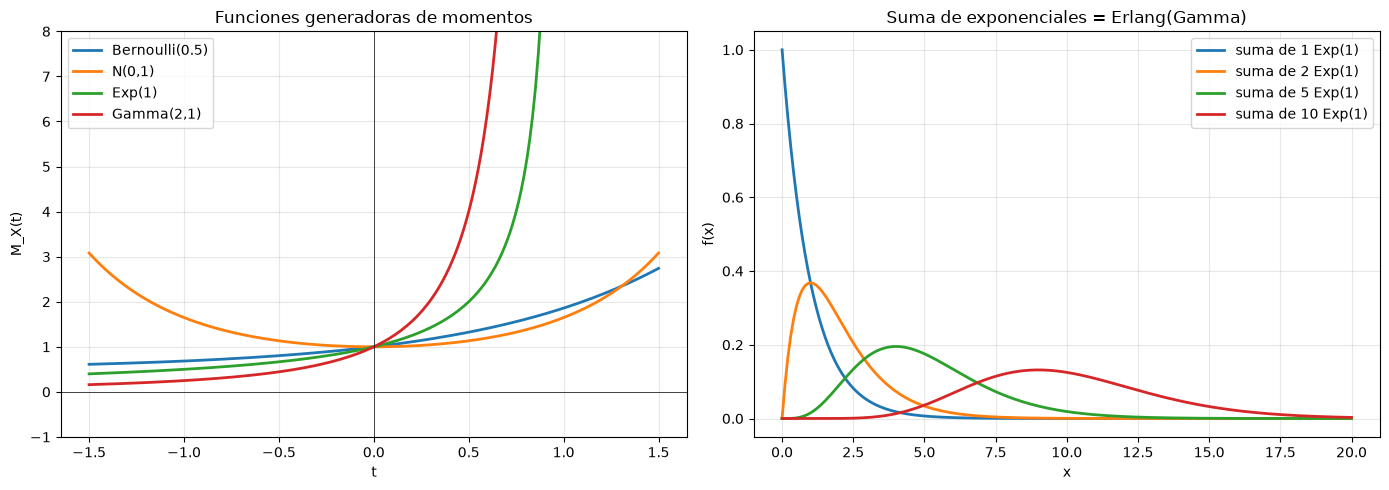
\includegraphics[height=7cm,keepaspectratio=true]{./pe/fgmDistribuciones.png}
 % fgmDistribuciones.png: 0x0 pixel, 300dpi, 0.00x0.00 cm, bb=
 \caption{Funciones generadoras de momentos y suma de variables gamma independientes.}
 \label{fig:2.8.4}
\end{figure}

{Tabla resumen de FGMs}
\begin{center}
\begin{tabular}{|l|l|}
\hline
\textbf{Distribución} & \textbf{FGM $M_X(t)$} \\
\hline
Bernoulli$(p)$ & $(1-p) + p\,e^t$ \\
Binomial$(n,p)$ & $(1 - p + p\,e^t)^n$ \\
Poisson$(\lambda)$ & $\exp(\lambda(e^t - 1))$ \\
Geométrica$(p)$ & $\dfrac{p\,e^t}{1 - (1-p)e^t}$ \\
Exponencial$(\lambda)$ & $\dfrac{\lambda}{\lambda - t}$ \\
Normal$(\mu, \sigma^2)$ & $\exp\!\left(\mu t + \dfrac{\sigma^2 t^2}{2}\right)$ \\
Gamma$(\alpha, \beta)$ & $(1 - \beta t)^{-\alpha}$ \\
Chi-cuadrada$_\nu$ & $(1 - 2t)^{-\nu/2}$ \\
\hline
\end{tabular}
\end{center}

\begin{observacion}
La propiedad de suma para v.a. independientes se aplica fácilmente: si
$X_1, \dots, X_n$ son Bernoulli$(p)$ iid, entonces
$\sum X_i \sim \text{Binomial}(n,p)$ y
\begin{align}
 M_{\sum X_i}(t) = \prod_{i=1}^n M_{X_i}(t) = (1 - p + p\,e^t)^n,
\end{align}
que coincide con la FGM de la distribución binomial.
\end{observacion}
